\documentclass[tikz,border=10pt]{standalone}
\begin{document}
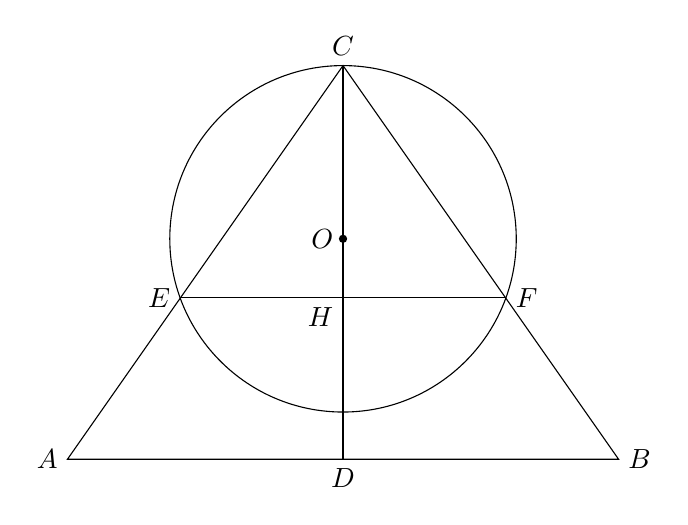
\begin{tikzpicture}
    % Define coordinates
    % Based on visual analysis:
    % Triangle ABC is isosceles with base AB on x-axis.
    % C is at (0, 5).
    % D is at (0, 0), foot of altitude.
    % A is at (-3.5, 0), B is at (3.5, 0).
    % Circle passes through C, centered at O on CD.
    % O is at (0, 2.8), Radius = 2.2 (so it passes through C(0,5)).
    % Bottom of circle is at y = 0.6, so it is above D(0,0).
    % E and F are intersections of circle with AC and BC.
    % H is intersection of EF and CD.
    
    \coordinate (A) at (-3.5, 0);
    \coordinate (B) at (3.5, 0);
    \coordinate (C) at (0, 5);
    \coordinate (D) at (0, 0);
    \coordinate (O) at (0, 2.8);
    
    % Approximate coordinates for E, F, H derived from geometry
    % E is approx (-2.07, 2.05)
    % F is approx (2.07, 2.05)
    % H is (0, 2.05)
    \coordinate (E) at (-2.07, 2.05);
    \coordinate (F) at (2.07, 2.05);
    \coordinate (H) at (0, 2.05);

    % Draw triangle ABC
    \draw (A) -- (B) -- (C) -- cycle;
    
    % Draw circle centered at O passing through C
    \draw (O) circle [radius=2.2];
    
    % Draw altitude CD
    \draw (C) -- (D);
    
    % Draw chord EF
    \draw (E) -- (F);
    
    % Label points
    \node[left] at (A) {$A$};
    \node[right] at (B) {$B$};
    \node[above] at (C) {$C$};
    \node[below] at (D) {$D$};
    \node[left] at (E) {$E$};
    \node[right] at (F) {$F$};
    \node[left] at (O) {$O$};
    \node[below left] at (H) {$H$};
    
    % Mark center O with a dot
    \fill (O) circle (1.5pt);
\end{tikzpicture}
\end{document}
